\documentclass[conference]{IEEEtran}
\IEEEoverridecommandlockouts
% The preceding line is only needed to identify funding in the first footnote. If that is unneeded, please comment it out.
\usepackage{cite}
\usepackage{amsmath,amssymb,amsfonts}
\usepackage{algorithmic}
\usepackage{graphicx}
\usepackage{textcomp}
\usepackage{xcolor}
\def\BibTeX{{\rm B\kern-.05em{\sc i\kern-.025em b}\kern-.08em
    T\kern-.1667em\lower.7ex\hbox{E}\kern-.125emX}}
\begin{document}

\title{Chess Assignment\\
{\footnotesize Introduction to Reinforcement Learning (Spring 2022)}
}

\author{
    \IEEEauthorblockN{van den Bergh Laurin}
    \IEEEauthorblockA{\textit{Institute of Informatics} \\
    \textit{University of Zurich}\\
    Zurich, Switzerland \\
    laurin.vandenbergh@uzh.ch\\
    16-744-401}
}

\maketitle

\begin{abstract}
    % todo: remove red color
    \color{red}
    This document is a model and instructions for \LaTeX.
    This and the IEEEtran.cls file define the components of your paper [title, text, heads, etc.]. *CRITICAL: Do Not Use Symbols, Special Characters, Footnotes, 
    or Math in Paper Title or Abstract.
\end{abstract}

\begin{IEEEkeywords}
    % todo: remove red color
    \color{red}
    reinforcement learning, chess
\end{IEEEkeywords}






\section{Introduction}\label{sec:introduction}

In this assignment, we explore the use of reinforcement learning algorithms to learn how to win a simplified version of chess. This version of chess takes place on a 4 by 4 board and can be thought of as a late game, where the agent has a king and a queen and the opponent only has a king. Since this game can only end in a win for the agent or in a draw, it is the agent's goal to learn how to win the game and avoid draws. The agent will be given a reward of 1 for winning, 0 for drawing, and 0 for all intermediate steps.

We explore and compare three different reinforcement learning algorithms on this game, namely: Q-learning, SARSA, and DQN.


Even though I/we completed this assignment alone, I decided to answer some of the ``group only'' questions in the assignment, as they related to the algorithms I used.






\section{Methods}\label{sec:methods}

\textcolor{blue}{(1) Describe the algorithms Q-learning and SARSA. Explain the differences and the possible advantages/disadvantages between the two methods. No coding is needed to reply to this question.}

\subsection{Q-Learning and SARSA}

\textcolor{red}{explain algos: }Q-learning and SARSA are types of temporal-difference (TD) algorithms for learning -- or estimating -- Q-values from interaction with an environment through trial and error. Both algorithms can be used for any policy, such as in this case an $\epsilon$-greedy policy, and both address the value-assignment problem, that is trying to attribute future rewards to previous actions, these (not actually the rewards get discounted, but the q-value) get discounted with the hyper parameter $\gamma$.

\textcolor{red}{differences: }(they behave differently: cliff example) Both algorithms choose their first action according to their chosen policy, e.g. $\epsilon$-greedy. However, they differ in how they choose their second action which is then also used to update the Q-value of the first action (i.e. to compare the second action Q-value?). SARSA is an on-policy algorithm which means that it chooses the second action according to the same policy as it used for choosing the first action. Q-learning, on the other hand, chooses the second action greedily, i.e. it chooses the action for which it thinks is best at that point in time/training.

SARSA has a higher tendency to explore than Q-Learning, because for updating the Q values it does not assume optimal play for the following actions. Q-Learning on the other hand assumes optimal play for future actions when computing the loss/delta. Q-learning finds the optimal policy if the environment fulfills the Markov property, that is [explain Markov property].

\textcolor{red}{advantages/disadvantages: }

q learning taking optimal path, but sarsa taking riskier path. what does that mean for chess? does it show in the results? q-learning lower expected rewards because of riskier moves that lead to accidental draws?
shaping rewards changes the objective.

Implemented from scratch.

\textcolor{blue}{(3) [Group Only (mention implementation and related things only)] We provide you with a template code of the chess game. Fill the gaps in the
program file chess implementing either Q Learning or SARSA; detailed instructions
are available inside the file. We provide indicative parameter values. Produce two
plots that show the reward per game and the number of moves per game vs training
time. The plots will be noisy. Use an exponential moving average.}



\subsection{Experience Replay (and DQN)}

\textcolor{blue}{(2) [Group Only] Describe the experience replay technique. Cite relevant papers.}

Experience replay is the technique used in the DQN algorithm \cite{atari2013} which stores past experiences that can be used for later training. This essentially allows us to transform the learning process from online learning to mini-batch learning, which helps to combat unstable behavior when using Q-Learning with a neural network to approximate the value function. 

- transform online to minibatch learning -> supervised learning
- better convergence behavior bc data more iid (due to random sampling), i.e. data in a mini-batch is decorrelated, which is assumed in convergence proofs\\
- more stable learning \\
- reuse of past experiences multiple times -> can help to speed up convergence

In 

For DQN no sequence is needed, because chess fulfills Markov property and gives rise to a Markov Decision Process (MDP). Also no preprocessing of sequence is needed anymore because state encoding is already given. \cite{atari2013} \cite{dqn2015}


\textcolor{blue}{(5) Implement another Deep RL algorithm (it could be SARSA if you chose before Q
Learning and vice versa). Compare the new results with your previous results.}

Chess has/fulfills the Markov property, so applying reinforcement learning algorithms like Q-Learning and SARSA is theoretically justified.






\section{Results}\label{sec:results}

\textcolor{blue}{(3) We provide you with a template code of the chess game. Fill the gaps in the
program file chess implementing either Q Learning or SARSA; detailed instructions
are available inside the file. We provide indicative parameter values. Produce two
plots that show the reward per game and the number of moves per game vs training
time. The plots will be noisy. Use an exponential moving average.}

\begin{figure}
    \centering
    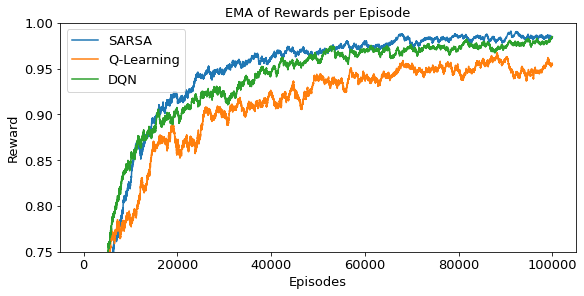
\includegraphics[width=.45\textwidth]{../figures/ema_rewards_per_episode_comparison.png}
\end{figure}

\begin{figure}
    \centering
    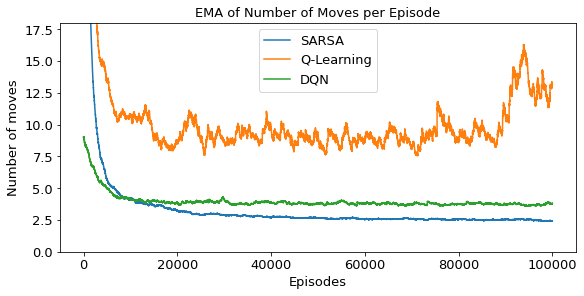
\includegraphics[width=.45\textwidth]{../figures/ema_number_of_moves_per_episode_comparison.png}
\end{figure}


\textcolor{blue}{(5) Implement another Deep RL algorithm (it could be SARSA if you chose before Q
Learning and vice versa). Compare the new results with your previous results.}

\subsection{Hyperparameters}

\textcolor{blue}{(4) Change the discount factor $\gamma$ and the speed $\beta$ of the decaying trend of $\epsilon$ (for a definition of $\beta$ please see code). Analyse the results.}

plot beta and gamma against performance metrics (maybe 3d). Interpret results.


\textcolor{blue}{(6) [Group Only] Change the state representation or the administration of reward. Interpret your results.}

\textcolor{blue}{(7) [Group Only] The values of the weights could explode during learning. This
issue is called exploding gradients. Explain one possible way to fix this issue and
implement it. For example, search and study RMSprop). Show in a plot how your
solution fixed this issue.}








\section{Conclusion}\label{sec:conclusion}



\section{Appendix}
% todo: remove red color
\textcolor{red}{put the appendix after the bibliography?}




\textcolor{red}{get correct bib format and complete entries}
\begin{thebibliography}{00}
    \bibitem{atari2013} V. Mnih, K. Kavukcuoglu, D. Silver, D. Wierstra, A. Graves, I. Antonoglou, M. Riedmiller , ``Playing Atari with Deep Reinforcement Learning.'', CoRR, vol
    % TODO: following entry is wrong
    \bibitem{dqn2015} V. Mnih, K. Kavukcuoglu, D. Silver, D. Wierstra, A. Graves, I. Antonoglou, M. Riedmiller , ``Playing Atari with Deep Reinforcement Learning.'', CoRR, vol

    % todo: remove red color
    \color{red}
    \bibitem{b1} G. Eason, B. Noble, and I. N. Sneddon, ``On certain integrals of Lipschitz-Hankel type involving products of Bessel functions,'' Phil. Trans. Roy. Soc. London, vol. A247, pp. 529--551, April 1955.
\end{thebibliography}
% todo: remove red color
\color{red}
\vspace{12pt}
IEEE conference templates contain guidance text for composing and formatting conference papers. Please ensure that all template text is removed from your conference paper prior to submission to the conference. Failure to remove the template text from your paper may result in your paper not being published.

\end{document}
